\documentclass[a4paper, titlepage]{article}
\usepackage[T1]{fontenc}
\usepackage[swedish]{babel}
\usepackage[utf8]{inputenc}
\usepackage{graphicx}
\usepackage[normalem]{ulem}
\title{
    Programming Project \\
    C++ Programming(EDA031)
}
\author{
        Department of Computer Science \\
            \\
        Simon Thörnqvist (ada09st1@student.lu.se)
            \and
        Fredrik Pettersson (ada09fpe@student.lu.se)
            \and
        Marcus LindFeldt (ada08mli@student.lu.se)
            \and
        [Robobuilder enter name and email here]
}
\date{\today}
\begin{document}
\maketitle

\section{Introduction}\label{introduction}
The purpose of this project was to implement a news system similar to the Usenet News. The assignment included the implementation of the server, the client and the communication between them. NNTP was the protocol used for the communication.

The news system contains articles which has a title, an author and text. Articles are created by the users of the system on the client side which are then stored on the server. Each created article is added to a newsgroup.

\section{Requirements}\label{requirements}
We believe that all requirements have been fulfilled.

\section{System Outline}\label{systemoutline}

\subsection{Com}
The package contains the protocol used for communication and the connection class for communication between client and server.

\subsubsection{MessageHandler}
The Message Handler is used to receive and send data via the communication socket. Both the server and the client use this class for sending / receiving commands.

\subsection{Database}

\subsubsection{In Memory}
This implementation of the database stores the information in the primary memory and destroys it when the server is terminated. It simply uses a map to store the newsgroups where the key is the id number of the newsgroup. Each newsgroup has it's own map to store their articles and the key is the id number of the article. Articles store the title, author and text as strings.

\subsubsection{File}
[Marcus insert knowledge here]

\subsection{Server}
 The server listens to a port, waiting for connections. When a conenction has been established it uses Message Interpreter and to intepret commands sent from the client. MessageHandler is used to receive and send data between the client and server. MessageHandler is used to receive and send data between the client and server.   

\subsubsection{Message Interpreter}
The protocol codes sent to the client are read in MessageIntepreter via the Message Handler. Depending on what code was sent different functions are called. When a code matches a code in the protocol a function is called, which calls a function in the database. The database returns a result and Message Interpreter inteprets the result and sends codes back to the client.

\subsubsection{Server Handler}
ServerHandler is the main class on the application server side. It uses the provided server class and utilizes the waitForActivity function to establish a connection with the client. When a connection has been established ServerHandler calls the MessageInterpreter function interpretAndPerform which reads the command from the client.

\subsection{Client}
[Robobuilder insert knowledge here]

\section{Communication}\label{communication}
[Flow chart of how the communication is carried out from inserting a command to the result printed out in the client]

\section{Summary}\label{summary}

\newpage
\appendix
\section{UML Diagram}\label{App:AppendixA}
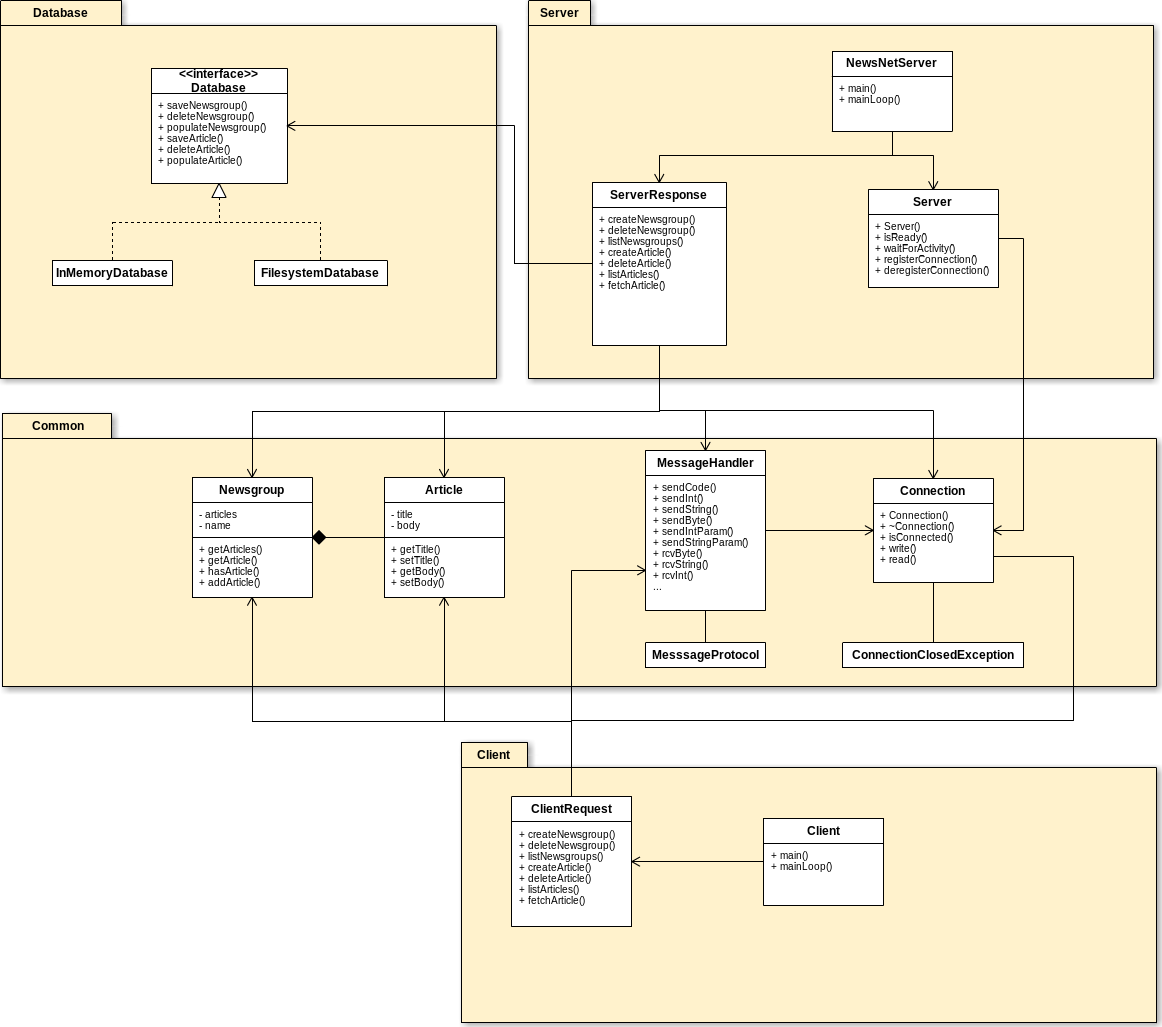
\includegraphics[width=130mm]{NewsNet_UML.png}

\end{document}